\section{Клиентская часть подсистемы аутентификации пользователей с применением
ПЦКД} 

В данной статье изложены технические аспекты и решения возможностей применения
портативных цифровых устройств для доступа в сети корпоративных порталов. В
частности, рассмотрены аппаратные особенности \textit{клиентской части} данной
системы доступа, как наиболее сложной с точки зрения организации, а также
сопутствующие программные средства и способы их интеграции для установления
взаимодействия между звеньями сложной цепочки компонентов системы.

\subsection{Технические особенности построения портативного цифрового устройства
доступа} 

В соответствии с предложенной методикой~\cite{concept_PCKD}, в качестве основной функции
ПЦКД выступает не только хранение идентификационных данных, но и непосредственное
участие в процессе генерации шифрограммы. Исходя из этого, следует, что
элементная база ПЦКД должна основываться на микропроцессорной системе, имеющей
аппаратный вычислитель.

В качестве ядра данной системы предлагается использовать 32-ух разрядный
микроконтроллер семейства AT91SAM7 от фирмы Atmel. Технические характеристики и
полный перечень особенностей приведен в таблицах описания для данного
микроконтроллера.~\cite{atmel}

Важно отметить следующие особенности данного микроконтроллера, которые
необходимы для решения всех аспектов поставленной задачи:
\begin{itemize}
  \item относительно малые размеры, позволяющие сделать устройство портативным;
  \item высокое быстродействие, применительно к возложенным функциям;
  \item невысокая стоимость, что позволит сделать продукт массовым;
  \item наличие порта устройства USB 2.0, позволяющего облегчить подключение к
  ПК;
  \item наличие  встроенных битов
блокировки и бита защиты, которые позволяют защитить прошивку микроконтроллера
от несанкционированной перезаписи или хищения, что немаловажно в задачах
криптографии.
\end{itemize}

При проектировании ПЦКД была разработана схема электрическая принципиальная
(см. Приложение~\ref{pril:A}, рисунок~\ref{ris:cxeme}), основа которой предложена на
официальном сайте разработчика микроконтроллера.~\cite{olimex}

\subsection{Протокол взаимодействия ПК и ПЦКД}

Немаловажной составляющей предложенной методики является выбор протокола для
информационного обмена между ПК и ПЦКД. Основными критериями для выбора
протокола являются:
\begin{itemize}
  \item возможность реализации протокола выбранным микроконтроллером;
  \item высокая
надежность и скорость передачи данных по интерфейсу;
\item возможность создания
коммуникации между ПК и ПЦКД, используя известные методы и подходы.
\end{itemize}

Исходя из поставленных требований, в качестве протокола для взаимодействия ПК и
ПЦКД был выбран протокол USB HID. HID-устройства (Human Interface Device) это
устройства взаимодействия компьютера и человека, такие как:
\begin{itemize}
  \item клавиатуры, мыши, джойстики и другие указатели;
  \item игровые
рулевое управление и педали;
\item кнопки, переключатели, регуляторы; 
\item различные датчики и считыватели;
 \item и т. п.
\end{itemize}

Принципиально на основе HID-технологии можно организовать взаимодействие с любым
устройством, даже если оно не является в строгом смысле интерфейсным устройством
человека и компьютера.

На стороне хоста обменом с устройством будет руководить стандартный
 HID-драйвер, включенный в поставку операционной системы.

Максимально возможная скорость передачи данных при такой организации обмена
составляет 64 Кбит/сек. Такой показатель в сравнении с 12 Мбит/сек полной
скорости USB-шины является большим минусом HID-технологии в вопросе выбора
конкретной USB-реализации. Однако, для поставленной задачи указанной скорости
вполне хватает. Беря во внимание размерности параметров алгоритмов шифрования,
максимальное количество данных, передаваемых по USB интерфейсу равна 4 Кбайт в
обоих направлениях, следовательно, для передачи данных потребуется менее 500 мс.

При разработке HID-устройства необходимо обеспечить следующие требования,
налагаемые спецификацией:
\begin{itemize}
  \item полноскоростное HID-устройство может передавать 64000 байт каждую секунду: по
64 байта каждые 1 мс; низкоскоростное HID-устройство имеет возможность передать
вплоть до 800 байт в секунду: по 8 байт каждые 10 мс;
\item HID-устройство может
назначить частоту своего опроса для определения того, есть ли у него свежие
данные для передачи;
\item обмен данными с HID-устройством осуществляется
посредством специальной структуры, называемой репортом (Report). Каждый
определенный репорт может содержать до 65535 байт данных. Структура репорта
имеет весьма гибкую организацию, позволяющую описать любой формат передачи
данных. Для того, чтобы конкретный формат репорта стал известен хосту,
микроконтроллер должен содержать специальное описание – дескриптор репорта;
\end{itemize}

HID-устройства должны иметь конечную точку
типа Interrupt IN и могут иметь конечную точку типа Interrupt OUT. С помощью них
устройство может выдавать данные хосту и получать их от него. Типы и направления
передач мы рассматривали в статье, посвященной основам организации USB-шины.
Обмен данными с HID-устройствами осуществляется при помощи репортов. Они бывают
двух типов:
\begin{itemize}
  \item INPUT- и OUTPUT-репорты используются для периодических передачи и приема
данных;
\item FEATURE-репорты обычно используются для установки различных
параметров и свойств, а также передачи других данных в тех случаях, когда
предположить периодичность появляния таких данных сложно. FEATURE-репорты бывают как
направления IN, так и направления OUT. Такие репорты передаются и принимаются
только по каналу нулевой конечной точки.
\end{itemize}

При идентификации HID-устройств хост определяет, что устройство относится к HID
классу по коду класса 0x03 в дескрипторе интерфейса. Кроме того, HID-устройства
имеют специальные дескрипторы. После того как хост определит, что устройство
принадлежит к HID классу, он передает управление устройством соответствующему
драйверу и обмен  ведется под его руководством.~\cite{kozlov}

Следуя данной спецификации интерфейса была предложена схема организации
программных компонентов для обеспечения информационного обмена между ПК и ПЦКД,
показанная на рисунке~\ref{ris:3.3.1}.

\begin{figure}[h!]
\center{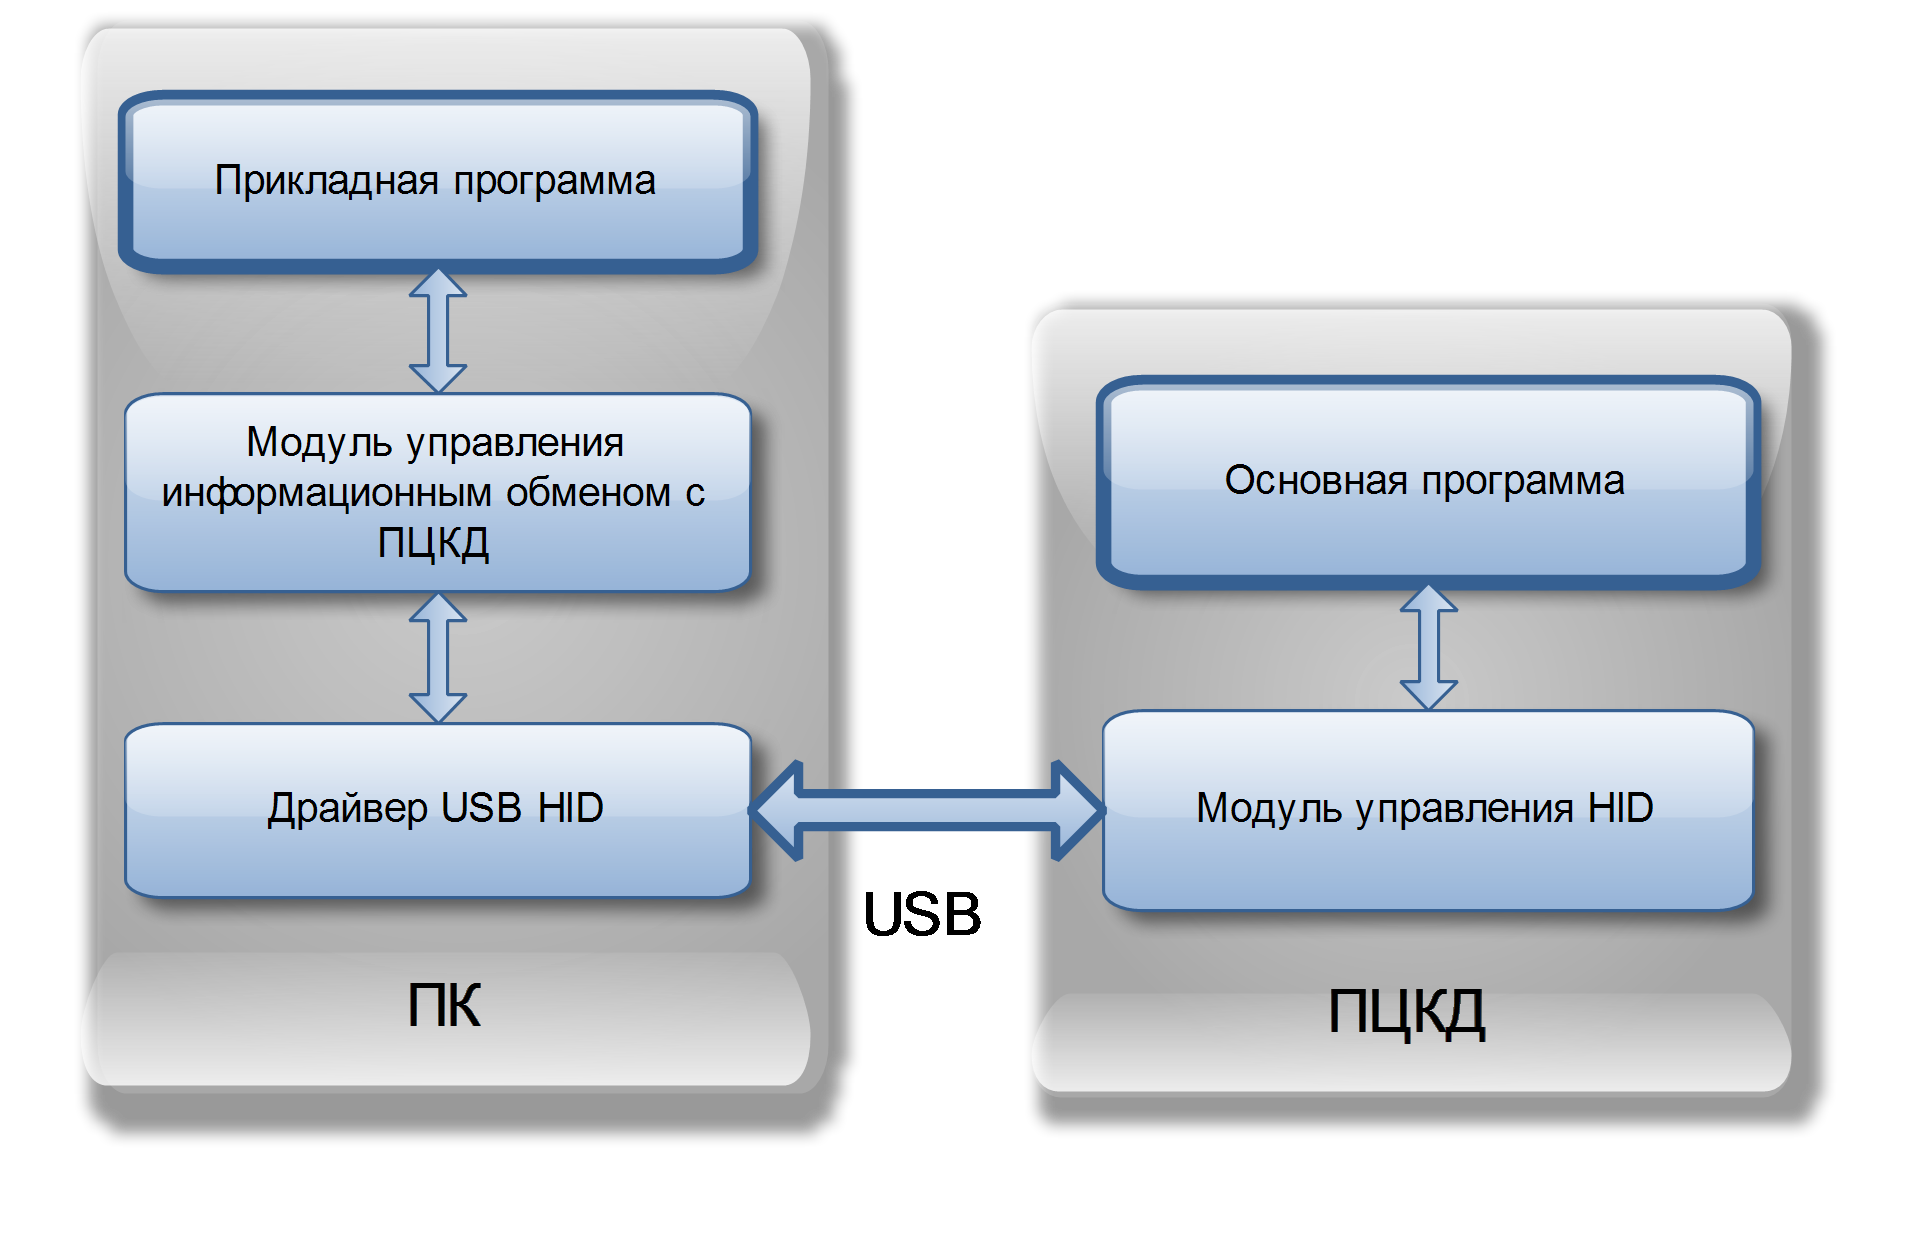
\includegraphics[width=1\linewidth]{3-3-1}}
\caption{Схема организации программных компонентов, обеспечивающих передачу
данных между ПК и ПЦКД с помощью USB HID}
\label{ris:3.3.1}
\end{figure}
 
На схеме представлены две основных программы, выполняющие целевую функцию и
взаимодействующие между собой: для ПК -- \textit{Прикладная программа}, для ПЦКД
-- \textit{Основная программа}. Остальные компоненты необходимы для
осуществления взаимодействия устройств через HID интерфейс. Модули управления
имеют набор функций, которые предназначены для приёма/передачи сообщений.

\subsection{Подходы к организации доступа к локальным ресурсам ПК из браузера}

Исходя из поставленной задачи, доступ к серверу должен осуществляться по
протоколу HTTP/HTTPS для максимального облегчения в использовании, а,
следовательно, все процессы по аутентификации пользователя на web-портале должны
быть инициированы браузером, выполняться в его рабочем пространстве и
контролироваться им. Согласно предложенной методике, часть действий, необходимых
для аутентификации, должны выполняться ресурсами ПЦКД. Возникает ситуация, при
которой необходимо создать механизм двустороннего взаимодействия с ПЦКД
средствами интернет-технологий, которые позволяют выполнять сценарии на стороне
клиента. Таким образом, схема организации программных компонентов
(рисунок~\ref{ris:3.3.1}) получает новую интерпретацию, где в роли прикладной
программы выступает браузер или сценарий, работающий под его управлением –
web-сценарий (рисунок~\ref{ris:3.3.2}).

\begin{figure}[h!]
\center{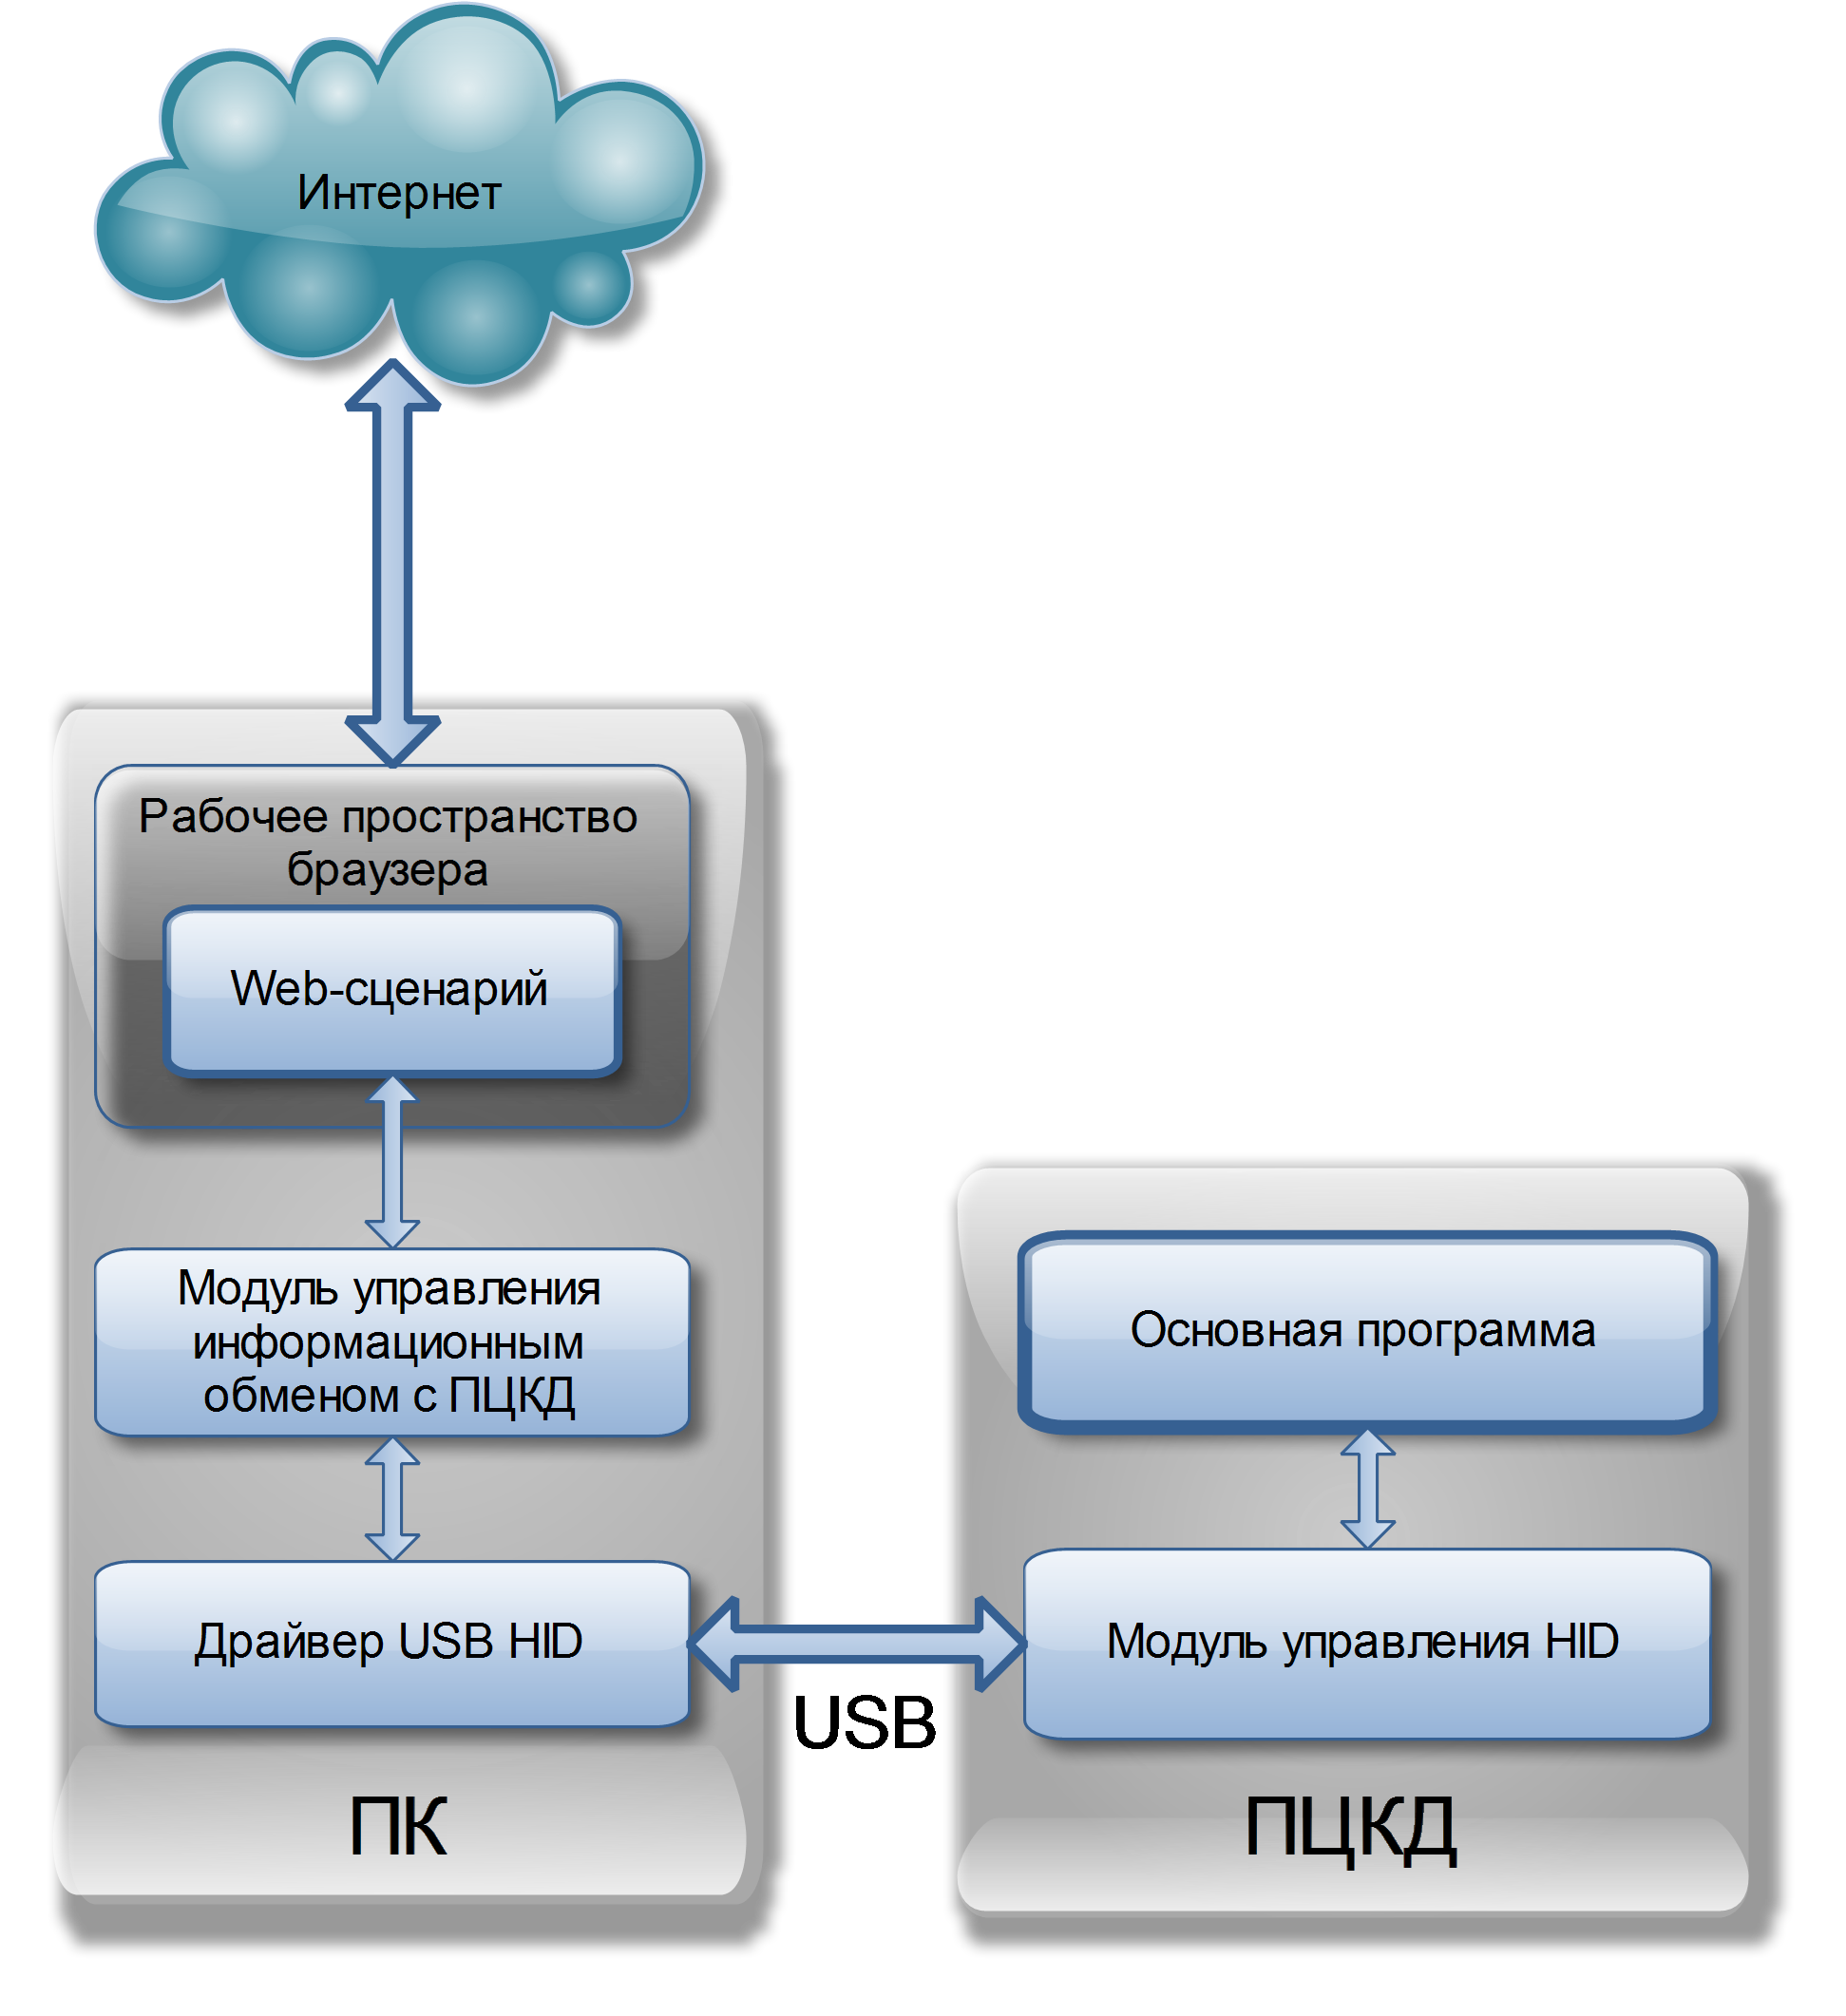
\includegraphics[width=1\linewidth]{3-3-2}}
\caption{Схема организации программных компонентов обеспечивающих передачу
данных между ПК и ПЦКД через браузер}
\label{ris:3.3.2}
\end{figure}

Данная схема весьма затруднительна с точки зрения её реализации, поскольку
возникает противоречие. С одной стороны, в соответствии с данной схемой,
взаимодействие с ПЦКД необходимо производить через драйвер ОС, относящийся к
локальным ресурсам ПК и являющийся внешним окружением по отношению к браузеру. С
другой стороны, браузер является средством доступа в глобальную сеть и имеет
мощные средства защиты от несанкционированного доступа к локальным ресурсам ПК,
и пресекает любые попытки обращения к ним.

Таким образом, возникает проблема, при которой необходимо получить доступ к
локальным ресурсам средствами браузера, что не позволяет делать его политика
безопасности.

Решение данной проблемы может получить развитие в следующих направлениях:
\begin{itemize}
  \item Создание модуля для браузера (плагина);
  \item Создание Java-апплета;
  \item Создание прикладной программы для ОС, которая будет работать независимо
  и выступать в роли посредника между web-сценарием и модулем взаимодействия с
  ПЦКД.
\end{itemize}

При анализе данных подходов были выявлены достоинства и недостатки каждого из
них в контексте проблемы, описанной выше. Полученные результаты зафиксированы в
таблице~\ref{tab:1}.

\begin{table}[ht]
  \small
  \centering
  \begin{tabular}{|p{3cm}|p{6cm}|p{7cm}|}
    \hline
	\textbf{Название технологии} & \textbf{Преимущества} & \textbf{Недостатки} \\
	\hline 
	\textit{Плагин для браузера} & полная интеграция с ОС на низком уровне, что
	упрощает механизм взаимодействия с ПЦКД & неудобство в использовании:
	\begin{itemize}
	  \item необходимость в отдельной установке;
	  \item для каждой версии браузера -- свой плагин.
	\end{itemize}  \\ \hline
	\textit{Java-апплет} & полная совместимость со всеми браузерами & получение
	доступа к локальным ресурсам возможно только после доверительного подписания апплета \\
	\hline 
	\textit{Независимая прикладная программа-посредник} & полная интеграция с ОС на
	 низком уровне, что упрощает механизм взаимодействия с ПЦКД & требует
	 дополнительной установки и сильно осложняет общий механизм взаимодействия
	 компонентов \\ \hline
  \end{tabular}
  \caption{Результаты сравнительного анализа предложенных технологий}
  \label{tab:1}
\end{table}

Следует так же отметить, что все рассмотренные
технологии позволяют в той или иной степени получать доступ к локальным ресурсам
ПК, там самым частично решая описанную проблему.

При окончательном рассмотрении представленных технологий выбор сделан в пользу
создания Java-апплета, так как этот подход позволяет обойти возникшую проблему и
наиболее качественно и легко решить поставленную задачу.

\subsection{Взаимодействие программных компонентов с использованием технологии
JavaApplet. Механизм JNI}

Как известно, в стандартную комплектацию \textit{Java Runtime Environment} (JRE)
не входит какой-либо класс или метод, позволяющий осуществить доступ к
USB-порту.
Поэтому, необходимо реализовать библиотеку, которая будет иметь методы
взаимодействия с USB устройством и осуществлять посреднические функции между
Java-апплетом и драйвером USB.
Java-апплет будет осуществлять взаимодействие с библиотекой посредством
механизма \textit{Java Native Interface} (JNE).~\cite{oracle}  Это стандартный
механизм для запуска кода, под управлением виртуальной машины Java (JVM), который написан
на языках С/С++ или Ассемблера,  скомпонованный в виде динамических библиотек, и
позволяет не использовать статическое связывание. Это даёт возможность вызова
функции С/С++ из программы на Java, и наоборот. Исходя из этого, структура
компонентов системы приобретает следующий вид (рисунок~\ref{ris:3.3.3}).

\begin{figure}[h!]
\center{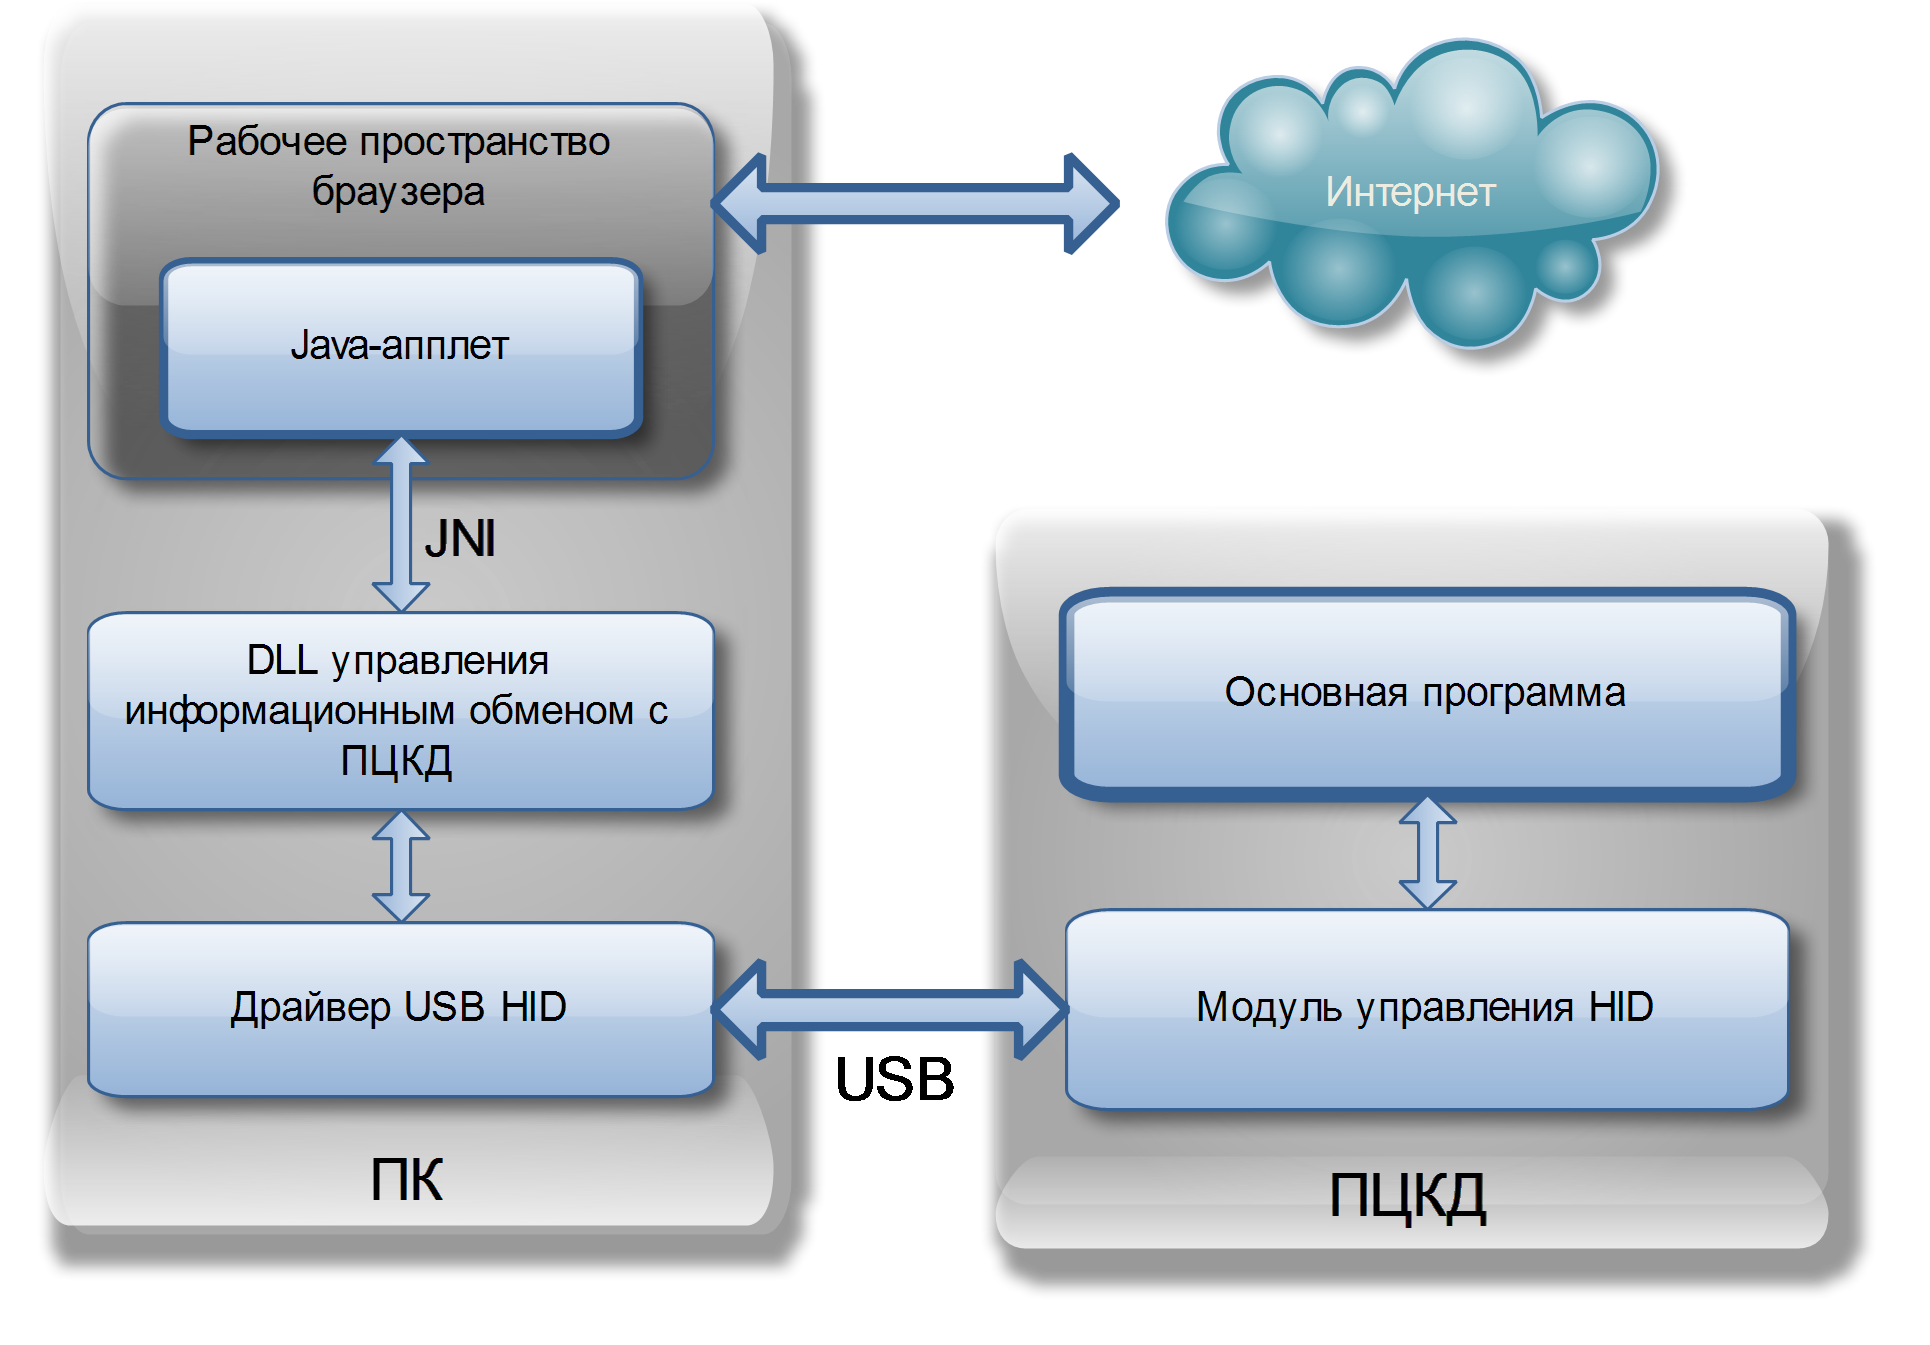
\includegraphics[width=1\linewidth]{3-3-3}}
\caption{Взаимодействие программных компонентов с использованием технологии
JavaApplet}
\label{ris:3.3.3}
\end{figure} 

Обязательным условием использования данного механизма является то, что
native-библиотека должна располагаться на диске машины клиента в специальной
директории. Следовательно, требуется инсталлировать библиотеку на
пользовательскую машину, после чего Java-апплет сможет подключить ее. Для этого
необходимо поместить Java-класс и библиотеку в jar-архив, который загрузится
вместе с html страницей. После чего, Java-апплет развернёт DLL-библиотеку во
временное хранилище машины пользователя и из него подгрузит DLL. Данную схему
иллюстрирует рисунок~\ref{ris:3.3.4}.

\begin{figure}[h!]
\center{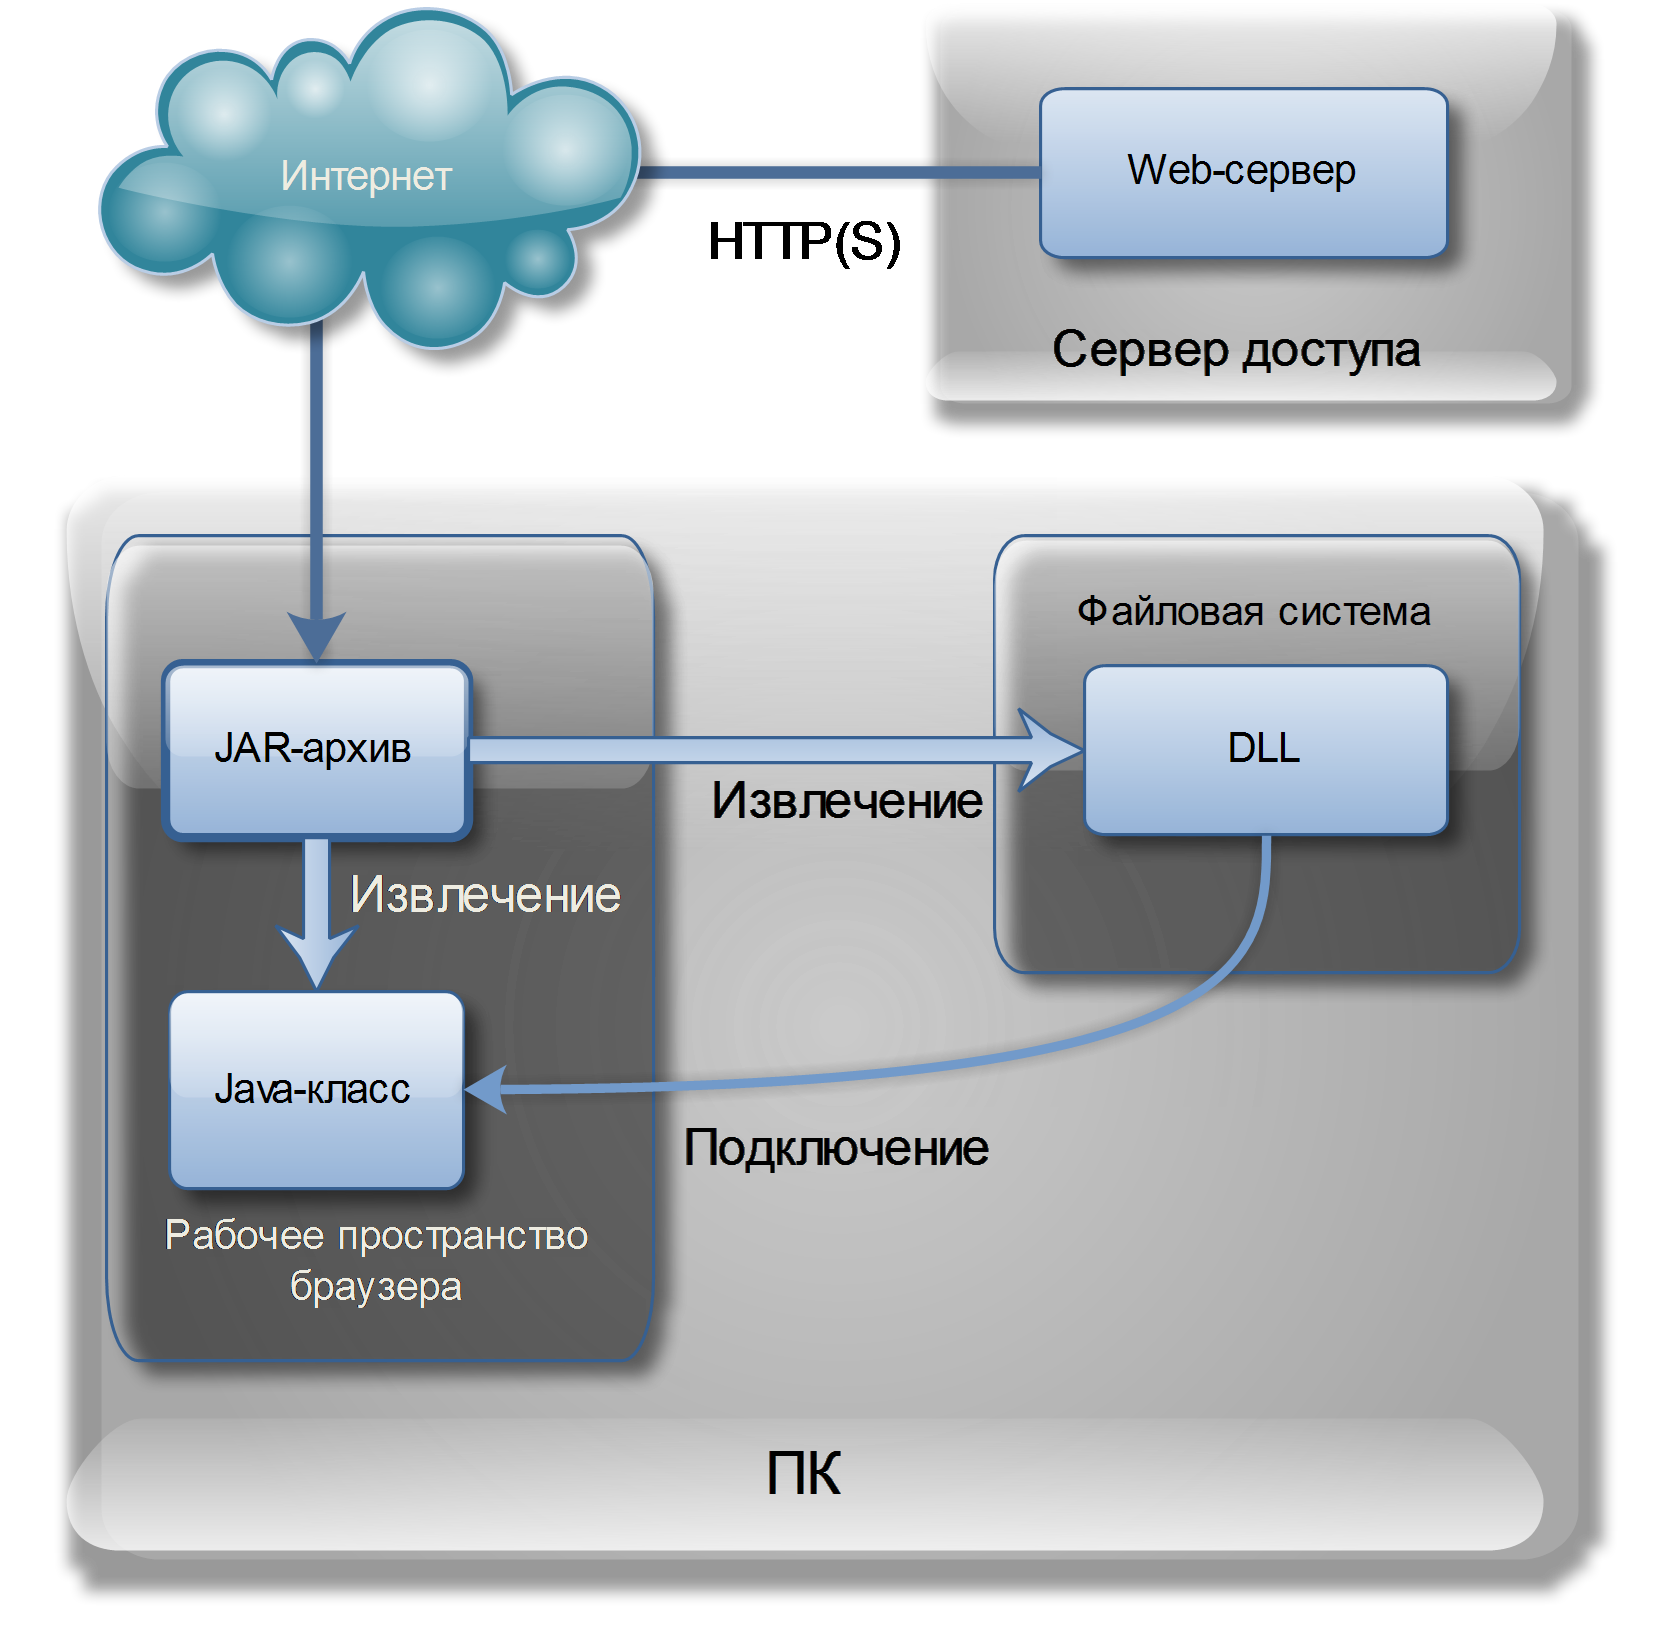
\includegraphics[width=1\linewidth]{3-3-4}}
\caption{Схема инсталляции библиотеки на клиентскую машину}
\label{ris:3.3.4}
\end{figure}  

В ходе развёртывания динамической библиотеки потребуется доступ к локальным
ресурсам пользователя (доступ к файловой системе). Java-апплету будет разрешён
доступ при условии его подписания электронно-цифровой подписью.~\cite{nikitin}

\subsection{Использование изложенных технических решений при построении системы доступа
к web-порталам с помощью ПЦКД}

В пункте~\ref{sect:concept} данной работы была рассмотрена схема
информационного обмена в процессе аутентификации пользователей в сети
корпоративных порталов.
Беря во внимание предложенные технические решения, упомянутая схема может быть
трансформирована в схему, приведенную на рисунке~\ref{ris:3.3.5}.
 
\begin{figure}[h!]
\center{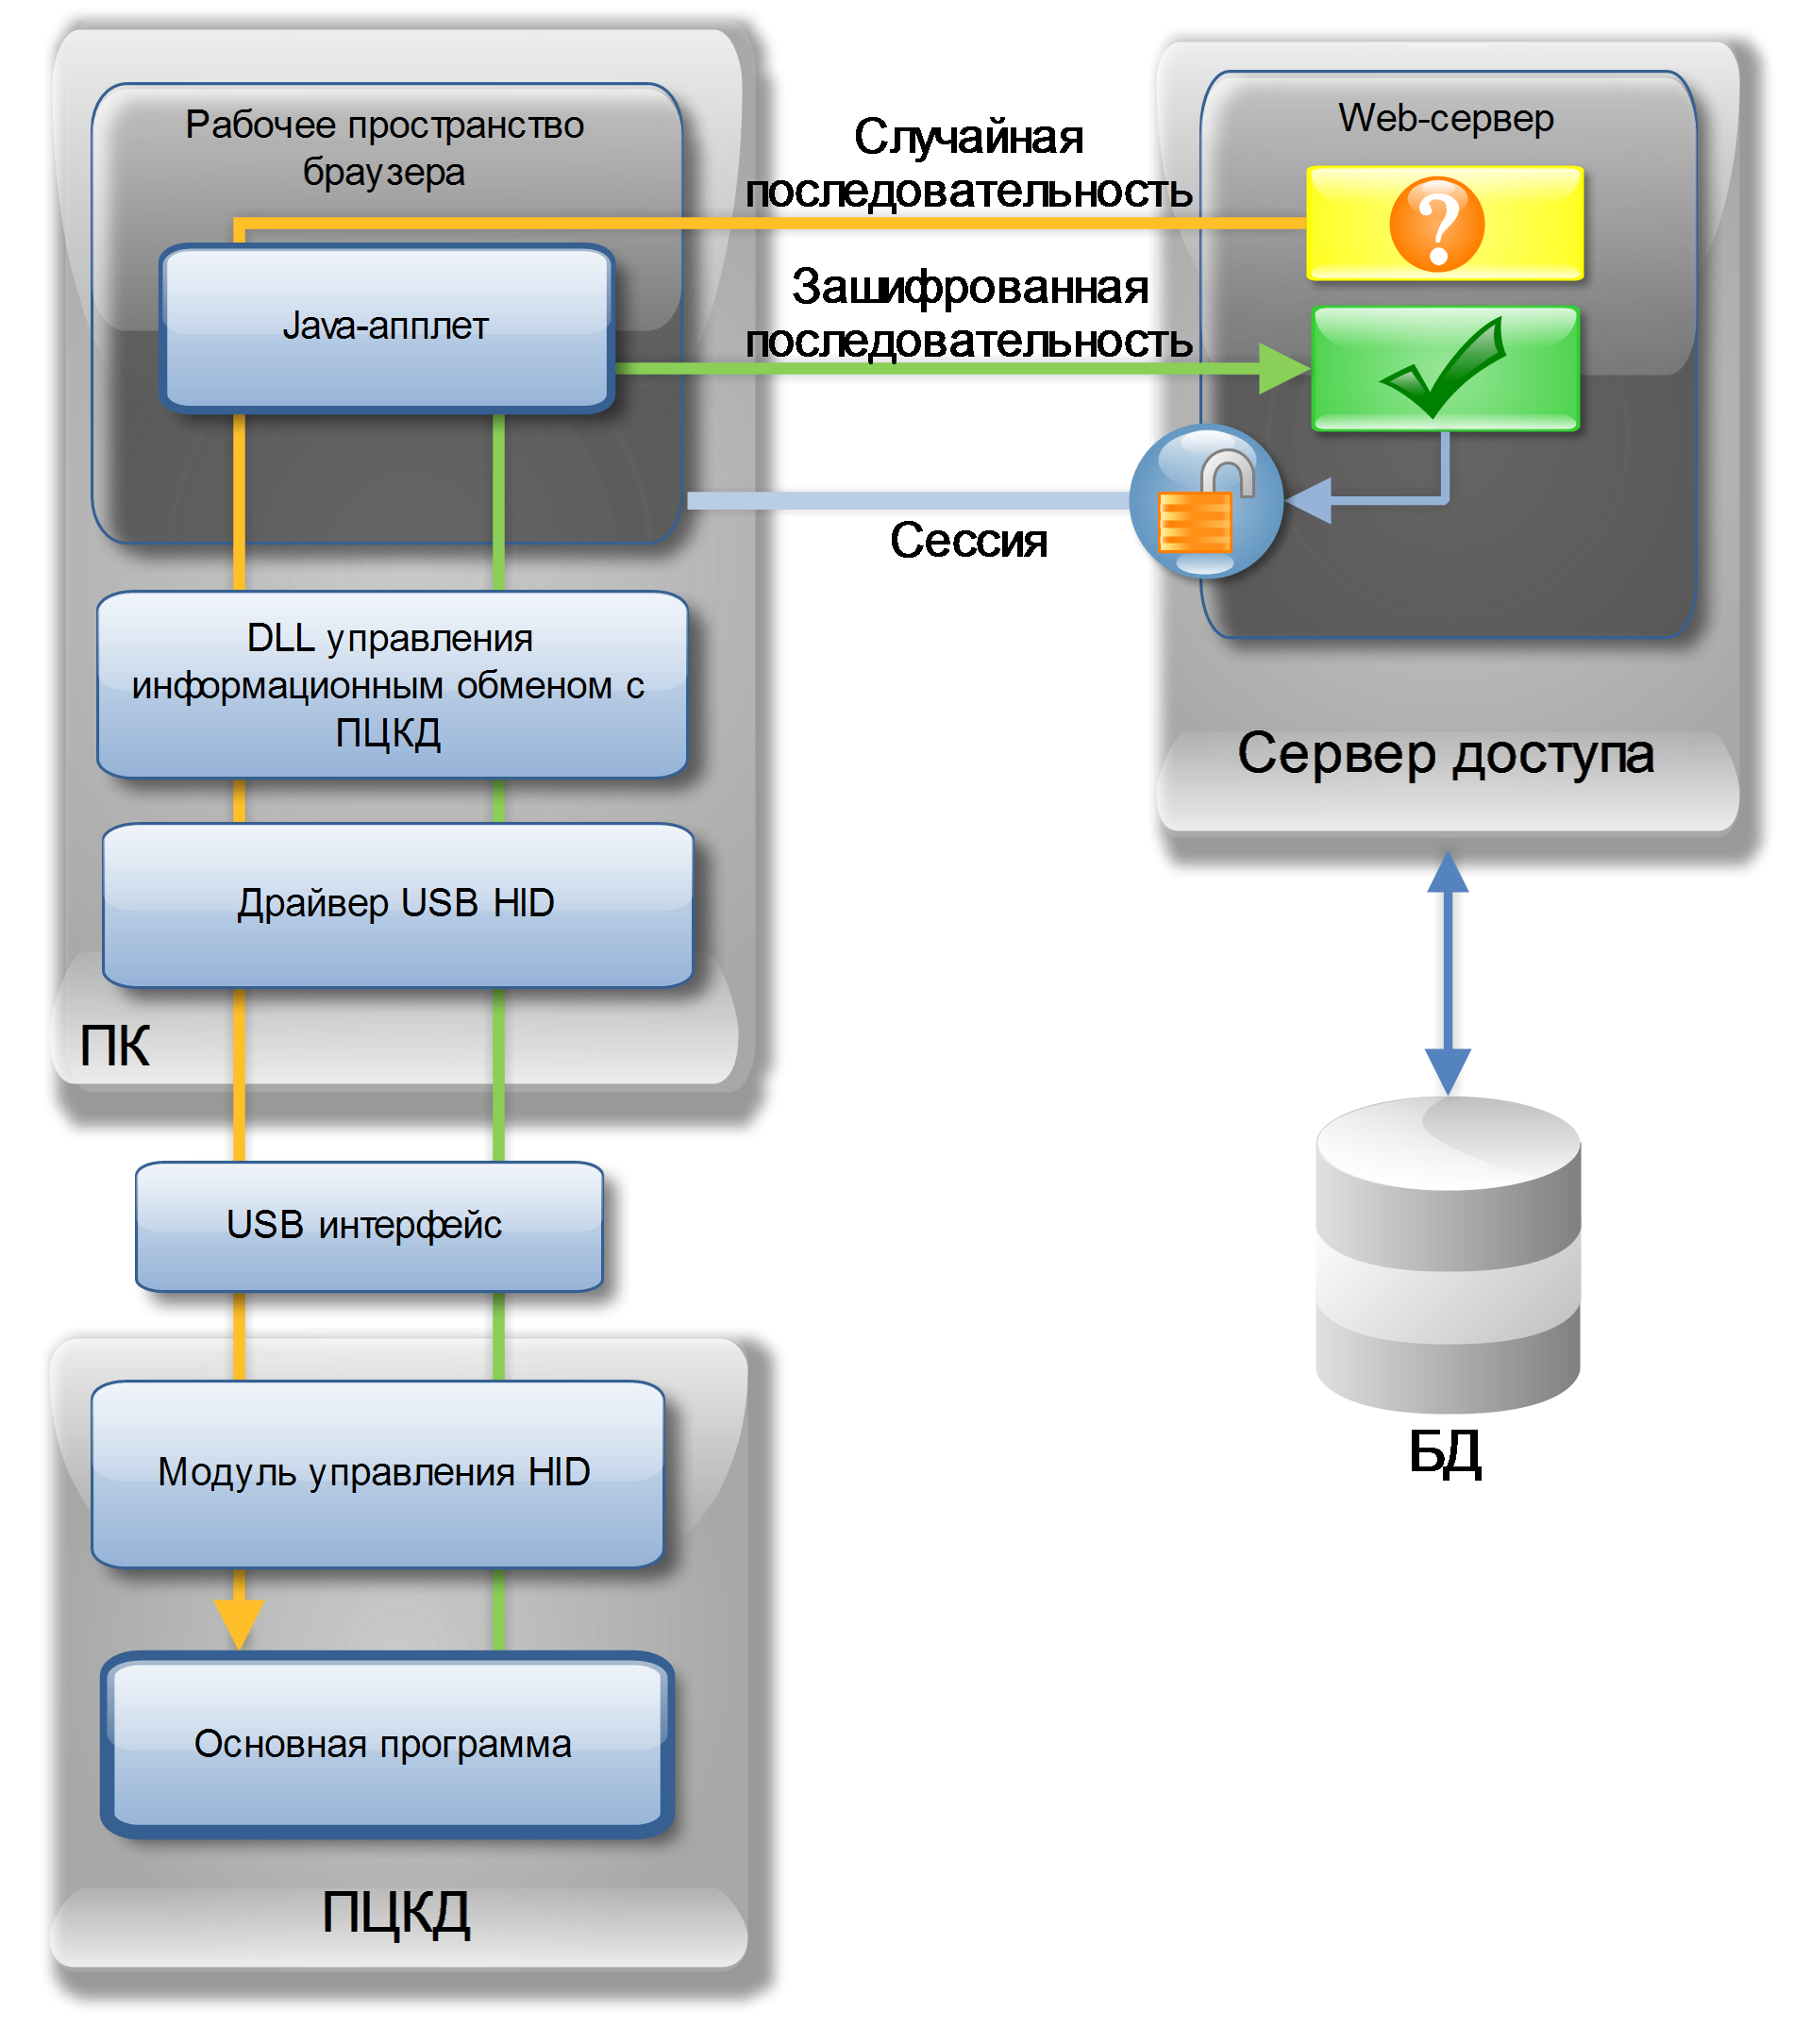
\includegraphics[width=1\linewidth]{3-3-5}}
\caption{Схема информационного обмена между пользователем и сервером доступа в
процессе аутентификации пользователей}
\label{ris:3.3.5}
\end{figure} 

При аутентификации пользователя в системе сервер отправляет случайную
последовательность битов, которые далее передаются в ПЦКД, реализуя предложенные
выше методы и технологии. После чего, ПЦКД шифрует полученную
последовательность, используя алгоритмы шифрования, а также секретный ключ, позволяющий однозначно
идентифицировать в системе пользователя – владельца ключа. Сгенерированный шифр
отправляется на сервер доступа, где проходит процедуру верификации. При
получении положительного ответа по окончании проверки, неизвестный признается
подлинным пользователем системы, в результате чего создаётся открытая сессия для
данного пользователя.~\cite{tex_asp}

\subsection{Описание протокола обмена данными высокого уровня с ПЦКД}

В соответствии с диаграммой активности, изображенной на
рисунках~\ref{ris:3.2.2}, ~\ref{ris:3.2.3}, а также, беря во
внимание схему на рисунке~\ref{ris:3.3.3} о взаимодействии программных и аппаратных компонентов
системы, можно утвержать, что существует необходимость в передаче разнородной
информации между ПК и ПЦКД.

Учитывая, что обмен данными по протоколу USB-HID осущаствляется через буфер,
который представляет собой массив байтов, возникает необходимость разработки
специального протокола обмена.

Исходя из функциональных требований к разрабатываемой подсистеме, можно выделить
действия, выполняемые ПЦКД:
\begin{enumerate}
  \item Получение от сервера, обработка и хранение секретного ключа;
  \item Вычисление сигнатуры (шифра) сообщения, полученного от сервера.
\end{enumerate}

В общем случае протокол входных данных можно представить в виде двух множеств:
$F$ -- множество функций и $P$ -- множество аргументов функций. Для каждой функции множество
аргументов $P$ может варьироваться. Множество $P$, в свою очередь,
трансформируется в тройку (формула~\ref{eq:set0}):

\begin{equation}
\label{eq:set}
<Q, S, D> ,
\end{equation}

где $Q$ -- множество параметров;

$S$ -- множество, значение ктоторого представлены в виде пары \textit{номер
аргумента -- размер в байтах};

$D$ -- множество аргументов;

\begin{equation}
\label{eq:set0}
\overbrace{f}^F \overbrace{\underbrace{q_1,q_2, \mbox{... } q_n}_Q
\underbrace{s_1,s_2, \mbox{... } s_m}_S \underbrace{(d_{1 1},d_{1 2}, \mbox{... }
d_{1 s_1});(d_{2 1},d_{2 2}, \mbox{... } d_{2 s_2}); \mbox{... } (d_{l 1},d_{l
2}, \mbox{... } d_{l s_m})}_D }^P
\end{equation}

Множества содержат незаконченый перечень значений.
Для первой функции (получение от сервера, обработка и хранение секретного
ключа) указанные подмножества (формула~\ref{eq:set}) могут принимать следующие
значения:

$Q = <q_1>$, где $q_1$ -- номер выбранного алгоритма шифрования;   

$D = <d_1, d_2>$, где $d_1$ -- шифр секретного ключа, $d_2$ -- идентификатор
пользователя в системе;

$S = <s_1, s_2>$, где $s_1$ и $s_2$ -- размер данных $d_1$ и $d_2$
соответственно.


Для второй функции (вычисление сигнатуры (шифра) сообщения, полученного от
сервера) подмножества аргументов~\ref{eq:set} могут принимать следующие
значения:

$D = <d_1>$, где $d_1$ -- сообщение, полученное клиентом;

$S = <s_1>$, где $s_1$ -- размер данных $d_1$.